\subsection{The evidence trail: miscitations, retractions and database attachment errors}\label{sec:dd-cite}
\textbf{Claim.} A citation can pass every mechanical check and still be wrong; and annotations
outlive their papers.
\textbf{Corpus.} Reviewers adjudicated \nRefReviews{} references: \pctRefVerified\% verified, \nRefMiscited{}
miscited (right paper, wrong claim), \nRefWrongIdentifier{} resolving to the wrong paper, \nRefDisputed{} disputed
and \nRefLowQuality{} low quality (Fig.~\ref{fig:evidencetrail}c). \nSourceDefects{} defects in source records on
\nSourceDefectGenes{} genes are filed for upstream correction, \pctDefectWrongTerm\% of them a wrong term and the
rest wrong gene products, evidence codes, qualifiers, references and WITH/FROM values (Fig.~\ref{fig:evidencetrail}a,b).
\begin{figure}[t]\centering
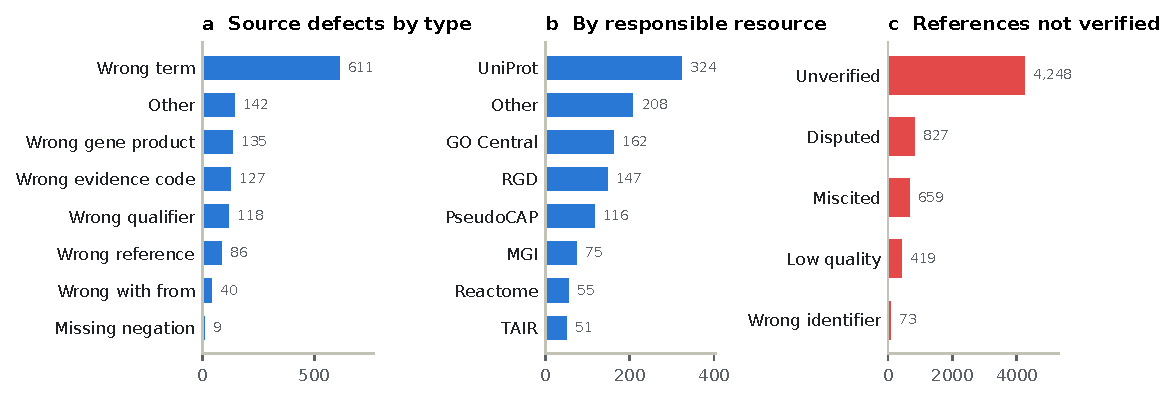
\includegraphics[width=\linewidth]{figures/evidence_trail.pdf}
\caption{The evidence trail. (a) Defects recorded in source annotation records, by type, and (b) by the
resource responsible. (c) Reference adjudications other than ``verified''.}
\label{fig:evidencetrail}
\end{figure}
\textbf{Data.} \proj{MISCITATIONS.md}: 14,559 adjudicated references, 559 flagged (enriched
sample); four of six seed cases are database attachment defects (wrong WITH/FROM, experimental
code on a meeting abstract, missing NOT). \proj{RETRACTIONS.md}: 25,088 PMIDs checked, 7 retracted,
13 expressions of concern; 4 retracted papers underlie GO annotations.
\textbf{External benchmark.} \proj{RAR\_MISANNOTATION.md}: of 290 pairs flagged by Wei et al.\
2020, 216 since removed from GOA, 38 persist; among survivors, plant lipid~A biosynthesis is
correct and the paper wrong. \note{Good calibration point: agentic review agrees with a prior
expert audit and corrects it where new evidence exists.}
\textbf{Upstream.} \texttt{source\_defects} $\rightarrow$ per-resource reports.
